\documentclass{article}
\usepackage{mathnotes}

\title{Regions of the Complex Plane}
\description{Definitions and properties of neighborhoods, interior and boundary points, open and closed sets, domains, and connectivity in the complex plane.}

\begin{document}

\section{Regions of the Complex Plane}

\begin{note}\label{complex-regions-overlap-note}
This overlaps with the definitions in \pagelink{metric-spaces} - I need to combine these!
\end{note}

An \textbf{$\epsilon$-neighborhood} of a point $z_0$ is the set of all \@{complex-numbers} $z$ satisfying

\[ | z - z_0 | < \epsilon. \]

This is the set of all complex numbers interior to a circle of radius $\epsilon$ and center $z_0$, but not including the circumference of the circle.

A point $z$ of a set $S$ of \@{complex-numbers} is called an \textbf{interior point} of $S$ if there exists an $\epsilon$-neighborhood of $z$ that contains only points of $S$.

On the other hand, $z$ is a \textbf{boundary point} of $S$ if every $\epsilon$-neighborhood of $z$ contains at least one point of $S$ and at least one point not in $S$. The set of all boundary points of a set $S$ is called the \textbf{boundary} of $S$.

A set $S$ of \@{complex-numbers} is said to be \textbf{open} if all points in $S$ are interior points. Alternatively, a set is open if it contains none of its boundary points.

A set $S$ of \@{complex-numbers} is said to be \textbf{closed} if it contains all of its boundary points.

Note that a set can be both open and closed! Both the empty set and $\complexes$ are both open and closed.

A set $S$ of \@{complex-numbers} is said to be \textbf{bounded} if there exists a positive (real) number $R$ such that $\|z\| < R$ for all $z$ in $S$. This means that a set is bounded if all its points fit within a circle of finite radius. A set that is not bounded is said to be \textbf{unbounded}.

\begin{definition}[Connected Complex]
A set $S$ is said to be \textbf{connected} if every pair of points in $S$ can be joined by a finite number of line segments joined end to end that lie entirely within $S$.
\end{definition}

\begin{definition}[Domain]
A \textbf{domain} is an \@{open} \@{connected} \@{set}. Note that this is not the same as a domain of definition of a function.
\end{definition}

In the images below, a dashed line represents a boundary that is not included the in the set, while a solid line represents a boundary that is included in the set.

Squiggly blue highlighter indicates the set goes on forever and the party never ends!

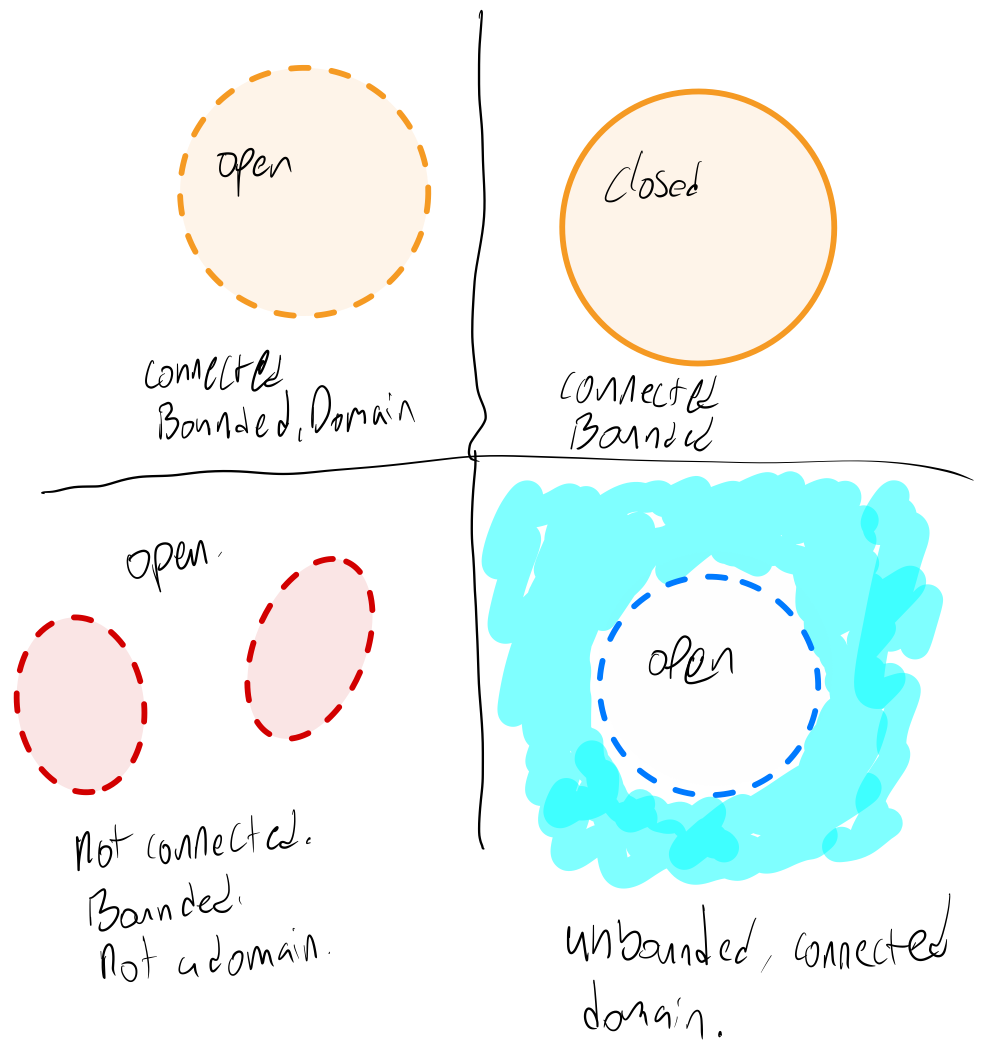
\includegraphics[alt={Regions of the Complex Plane}]{regions.png}

\end{document}
